\RequirePackage{fix-cm}
\documentclass{article}
\usepackage{lmodern}
\usepackage{mathtools}
\usepackage[paperwidth=190cm, paperheight=90cm, margin=0pt]{geometry}
\usepackage{amsmath, amssymb, booktabs, array, graphicx, colortbl}
\usepackage{tikz, pgfplots}
\pgfplotsset{compat=1.18}
\usepackage{algorithmic}
\usetikzlibrary{calc, positioning, arrows.meta}
\pagestyle{empty}

\definecolor{mkgreen}{RGB}{0,128,80}
\definecolor{mkgreenlight}{RGB}{232,245,238}
\definecolor{nmblue}{RGB}{50,100,180}
\definecolor{posterbg}{RGB}{245,247,249}
\definecolor{titlebg}{RGB}{13,72,52}

\graphicspath{{../Figures/}}
\newcommand{\wt}[1]{\overset{\scalebox{1.8}[1.0]{\raisebox{-3pt}{$\sim$}}}{#1}}

% Block: #1=name, #2=position, #3=width(cm), #4=title, #5=body
\newcommand{\posterblock}[5]{%
  \node[name=#1T, anchor=north west,
    fill=titlebg, text=white,
    font=\sffamily\bfseries\fontsize{48}{50}\selectfont,
    text width=#3 cm - 30pt, inner sep=15pt,
    rounded corners=5pt]
    at (#2) {#4};%
  \node[name=#1B, anchor=north west,
    fill=white, text=black,
    font=\fontsize{43}{46}\selectfont,
    text width=#3 cm - 30pt, inner sep=15pt,
    rounded corners=5pt]
    at (#1T.south west) {#5};%
}

% Column 1 & 3: 10% larger
\newcommand{\posterblockL}[5]{%
  \node[name=#1T, anchor=north west,
    fill=titlebg, text=white,
    font=\sffamily\bfseries\fontsize{55}{58}\selectfont,
    text width=#3 cm - 30pt, inner sep=15pt,
    rounded corners=5pt]
    at (#2) {#4};%
  \node[name=#1B, anchor=north west,
    fill=white, text=black,
    font=\fontsize{49}{54}\selectfont,
    text width=#3 cm - 30pt, inner sep=15pt,
    rounded corners=5pt]
    at (#1T.south west) {#5};%
}

% Column 3: 5% smaller than L
\newcommand{\posterblockM}[5]{%
  \node[name=#1T, anchor=north west,
    fill=titlebg, text=white,
    font=\sffamily\bfseries\fontsize{52}{55}\selectfont,
    text width=#3 cm - 30pt, inner sep=15pt,
    rounded corners=5pt]
    at (#2) {#4};%
  \node[name=#1B, anchor=north west,
    fill=white, text=black,
    font=\fontsize{47}{51}\selectfont,
    text width=#3 cm - 30pt, inner sep=15pt,
    rounded corners=5pt]
    at (#1T.south west) {#5};%
}

% Column 2: 10% smaller
\newcommand{\posterblockS}[5]{%
  \node[name=#1T, anchor=north west,
    fill=titlebg, text=white,
    font=\sffamily\bfseries\fontsize{42}{44}\selectfont,
    text width=#3 cm - 30pt, inner sep=15pt,
    rounded corners=5pt]
    at (#2) {#4};%
  \node[name=#1B, anchor=north west,
    fill=white, text=black,
    font=\fontsize{37}{39}\selectfont,
    text width=#3 cm - 30pt, inner sep=15pt,
    rounded corners=5pt]
    at (#1T.south west) {#5};%
}

\begin{document}
\begin{tikzpicture}[remember picture, overlay,
  shift={(current page.north west)},
  x=1cm, y=-1cm]

% Background
\fill[posterbg] (0,0) rectangle (190,90);

% Title bar
\fill[titlebg] (0,0) rectangle (190,8);
\node[anchor=west, text=white, font=\sffamily\bfseries, scale=6.5]
  at (3,2.4) {Markovian Transformers for Informative Language Modeling};
\node[anchor=west, text=white, font=\sffamily, scale=3.7]
  at (3,5.0) {Scott W.\ Viteri \quad Max Lamparth \quad Peter Chatain \quad Clark Barrett};
\node[anchor=west, text=white!80, font=\sffamily, scale=3.0]
  at (3,6.7) {Department of Computer Science, Stanford University};
\node[anchor=east, text=white, font=\sffamily\bfseries, scale=3.7]
  at (187,5.0) {ICLR 2026};

% 3 columns: 59cm each, 2cm gaps, 3cm margins
% col1: x=3   col2: x=64   col3: x=125

% ===================== COLUMN 1 =====================

\posterblockL{C1A}{3,9.5}{59}{Problem: CoT Is Not Load-Bearing}{%
Standard Chain-of-Thought can be altered without changing the answer, because the model still sees the question when generating one.

\vspace{0.3cm}
\centering
\begin{tikzpicture}[
  box/.style={rectangle, draw, rounded corners=4pt,
    minimum width=10cm, minimum height=2cm,
    font=\fontsize{42}{44}\selectfont, align=center},
  arrow/.style={->, line width=2pt, >={Latex[length=14pt, width=10pt]}}
]
\node[box, fill=blue!10] (Q) at (0,5.5) {Question};
\node[box, fill=orange!15] (C) at (0,2.8) {CoT};
\node[box, fill=green!15] (A) at (0,0.2) {Answer};
\draw[arrow] (Q) -- (C);
\draw[arrow] (C) -- (A);
\draw[arrow, red, dashed, line width=3pt] (Q.east)
  to[bend right=25] node[right, font=\fontsize{42}{44}\selectfont, text=red] {bypass} (A.east);
\end{tikzpicture}

\vspace{0.2cm}
\raggedright
\textbf{Goal:} not full faithfulness, but \textbf{informativeness}---the CoT should suffice to support the answer on its own.
}

\posterblockL{C1B}{$(C1AB.south west)+(0,1.2)$}{59}{Markovian Language Model}{%
$M=(\mathcal{O},\mathcal{S},\pi,u,s_1)$: $\pi$ predicts observations \textbf{from state alone}.

\vspace{0.3cm}
\centering
{\fontsize{40}{42}\selectfont\bfseries
\makebox[18cm]{Non-Markovian}\hfill
\makebox[18cm]{\color{mkgreen}Markovian (Ours)}\hfill
\makebox[18cm]{\color{nmblue}Autoencoder Analogy}}

\vspace{0.3cm}
\centering
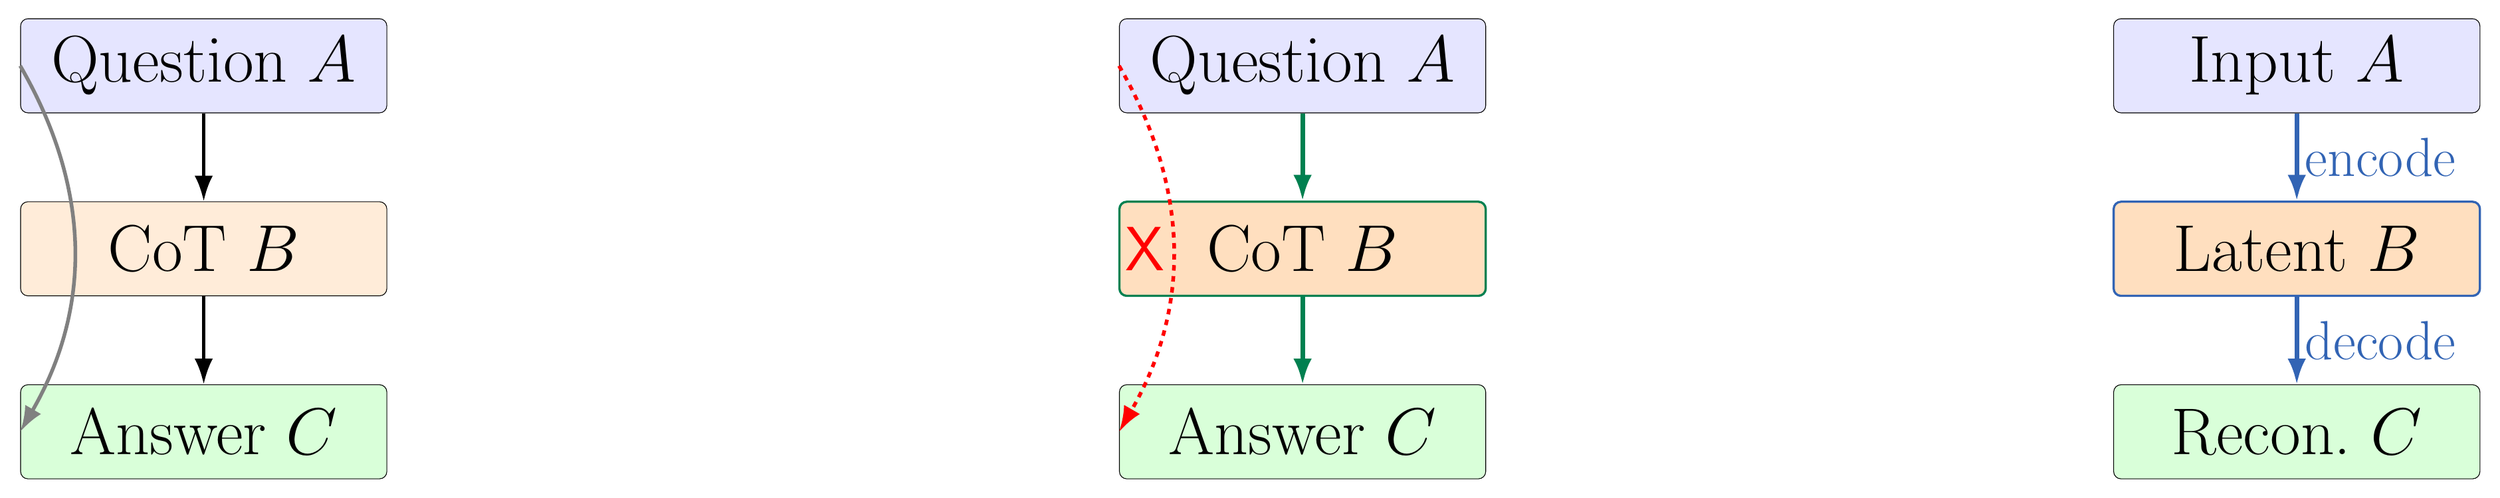
\begin{tikzpicture}[
  box/.style={rectangle, draw, rounded corners=4pt,
    minimum width=7cm, minimum height=1.8cm,
    font=\fontsize{36}{38}\selectfont, align=center},
  arrow/.style={->, line width=2pt, >={Latex[length=14pt, width=10pt]}}
]
\node[box, fill=blue!10] (Q1) at (-22,7) {Question $A$};
\node[box, fill=orange!15] (C1) at (-22,3.5) {CoT $B$};
\node[box, fill=green!15] (A1) at (-22,0) {Answer $C$};
\draw[arrow] (Q1) -- (C1);
\draw[arrow] (C1) -- (A1);
\draw[arrow, gray, line width=2pt] (Q1.west) to[bend left=30] (A1.west);

\node[box, fill=blue!10] (Q2) at (-1,7) {Question $A$};
\node[box, fill=orange!25, draw=mkgreen, very thick] (C2) at (-1,3.5) {CoT $B$};
\node[box, fill=green!15] (A2) at (-1,0) {Answer $C$};
\draw[arrow, mkgreen, line width=2.5pt] (Q2) -- (C2);
\draw[arrow, mkgreen, line width=2.5pt] (C2) -- (A2);
\draw[arrow, red, dashed, line width=2pt] (Q2.west) to[bend left=30]
  node[left, text=red, font=\fontsize{34}{36}\selectfont] {\textsf{X}} (A2.west);

\node[box, fill=blue!10] (E) at (18,7) {Input $A$};
\node[box, fill=orange!25, draw=nmblue, very thick, minimum width=7cm] (L)
  at (18,3.5) {Latent $B$};
\node[box, fill=green!15] (D) at (18,0) {Recon.\ $C$};
\draw[arrow, nmblue, line width=2.5pt] (E) -- node[right, font=\fontsize{30}{32}\selectfont]{encode} (L);
\draw[arrow, nmblue, line width=2.5pt] (L) -- node[right, font=\fontsize{30}{32}\selectfont]{decode} (D);
\end{tikzpicture}

\vspace{0.3cm}
\raggedright
All information from $A$ to $C$ must pass through bounded-length $B$: an \textbf{autoencoder-style reasoning bottleneck}.
}

\posterblockL{C1C}{$(C1BB.south west)+(0,1.2)$}{59}{Informativeness Objective \& Loss}{%
\textbf{Reward} (trained vs.\ frozen baseline):
\[
R_\theta = \ln \pi_\theta(\text{ans}\mid\text{CoT}) - \ln \pi'(\text{ans}\mid\text{CoT}')
\quad;\quad
J(\theta)=\mathbb{E}_{\tau}\!\left[R_\theta(\tau)\right]
\]
\vspace{-0.4cm}

\textbf{Gradient} (two terms because $R_\theta$ depends on $\theta$):
\[
\nabla_\theta J
= \mathbb{E}\!\left[
\underbracket{R_\theta \,\nabla_\theta \ln P_\theta}_{\text{policy gradient}}
+\;
\underbracket{\nabla_\theta R_\theta}_{\text{actor-reward}}
\right]
\]
\vspace{0.1cm}

\textbf{Loss:}\quad $\boxed{\;\mathcal{L}=\mathcal{L}_{\text{PG}}+\mathcal{L}_{\text{AR}}+\mathcal{L}_{\text{KL}}\;}$
\begin{align*}
\mathcal{L}_{\text{PG}} &= -\ln u_\theta(\text{CoT}\mid q)\cdot A^{\text{detach}}
  &&\text{(policy gradient)} \\
\mathcal{L}_{\text{AR}} &= -A
  &&\text{(actor-reward)} \\
\mathcal{L}_{\text{KL}} &= \beta_{\text{KL}}\,D_{\text{KL}}(u_\theta \,\Vert\, u')
  &&\text{(regularization)}
\end{align*}
}

% ===================== COLUMN 2 =====================

\posterblockS{C2A}{64,9.5}{59}{Training Algorithm}{%
\begin{algorithmic}[1]
\STATE \textbf{Given}: dataset $P$ of $(q,a)$, actor $(u_\theta,\pi_\theta)$, frozen baseline $(u',\pi')$
\FOR{each training batch of size $B$}
  \STATE \hspace{1.5em} Sample $(q,a) \sim P$
  \STATE \hspace{1.5em} Sample $\text{CoT}_i \sim u_\theta(\cdot\mid q,\text{CoT}_{\text{init}})$ for $i=1..B$
  \STATE \hspace{1.5em} Sample $\text{CoT}' \sim u'(\cdot\mid q,\text{CoT}_{\text{init}})$ \quad (frozen baseline)
  \STATE \hspace{1.5em} $r_i = \ln \pi_\theta(a\mid \text{CoT}_i)$;\enspace $b = \ln \pi'(a\mid \text{CoT}')$
  \STATE \hspace{1.5em} $R_i = r_i - b$;\enspace standardize: $A_i = (R_i - \mu)/(\sigma + \epsilon)$
  \STATE \hspace{1.5em} Compute $\mathcal{L}_{\text{PG}},\;\mathcal{L}_{\text{AR}},\;\mathcal{L}_{\text{KL}}$;\enspace update $\theta$
\ENDFOR
\end{algorithmic}
}

\posterblockS{C2B}{$(C2AB.south west)+(0,0.8)$}{59}{Main Result: Accuracy vs.\ Fragility}{%
Markovian training trades a few accuracy points for CoTs the model actually relies on.

\vspace{0.15cm}
\begin{minipage}[t]{25cm}
\centering
{\fontsize{41}{43}\selectfont\bfseries Accuracy}

\vspace{0.1cm}
\renewcommand{\arraystretch}{1.2}
\setlength{\tabcolsep}{4pt}
\begin{tabular}{l c c c}
\toprule
\textbf{Task} & \textbf{Base} & \textbf{NM} & \textbf{Mkv} \\
\midrule
GSM8K      & 19.6 & 63.3 & 57.1 \\
ARC        & 36.1 & 78.6 & 79.9 \\
Arith.     & 1.0  & 97.0 & 98.0 \\
MMLU       & 21.4 & 68.7 & 55.5 \\
SVAMP      & 18.0 & 43.3 & 42.3 \\
\bottomrule
\end{tabular}
\end{minipage}%
\hfill
\begin{minipage}[t]{29cm}
\centering
{\fontsize{41}{43}\selectfont\bfseries Perturbation}

\vspace{0.1cm}
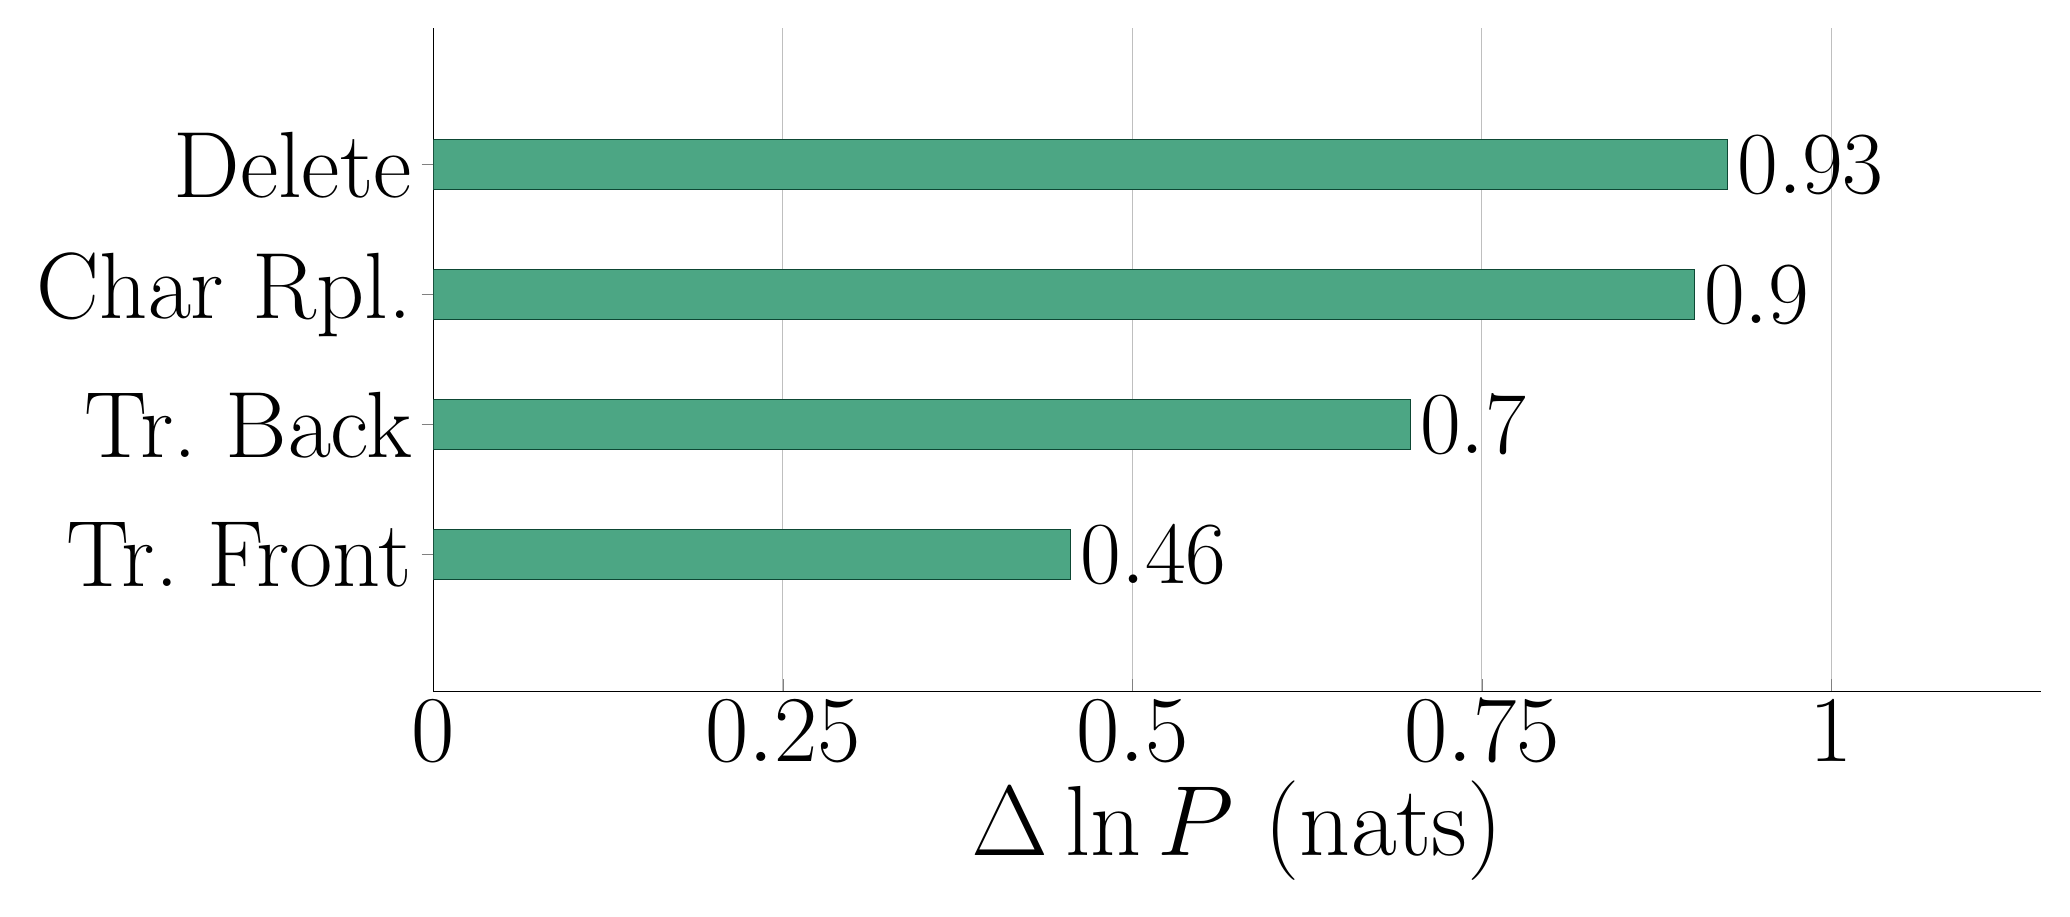
\begin{tikzpicture}
\begin{axis}[
  xbar, xmin=0, xmax=1.15,
  width=22cm, height=10cm,
  xlabel={$\Delta\ln P$ (nats)},
  xtick={0, 0.25, 0.5, 0.75, 1.0},
  symbolic y coords={TruncF,TruncB,CharRep,Del},
  ytick={TruncF,TruncB,CharRep,Del},
  yticklabels={Tr.\ Front, Tr.\ Back, Char Rpl., Delete},
  yticklabel style={font=\fontsize{34}{36}\selectfont},
  xticklabel style={font=\fontsize{34}{36}\selectfont},
  xlabel style={font=\fontsize{36}{38}\selectfont},
  nodes near coords,
  every node near coord/.append style={font=\fontsize{32}{34}\selectfont, anchor=west},
  xmajorgrids=true,
  axis y line*=left, axis x line*=bottom,
  bar width=18pt, enlarge y limits=0.35
]
\addplot[fill=mkgreen!70, draw=titlebg] coordinates {
  (0.456,TruncF) (0.699,TruncB) (0.902,CharRep) (0.926,Del)};
\end{axis}
\end{tikzpicture}
\end{minipage}

\vspace{0.1cm}
\textbf{Fragility:} ($\wt{\text{CoT}}$ = corrupted CoT)\par
\scalebox{1.0}{\parbox{53cm}{%
\begin{gather*}
\Delta = \underbracket{\ln\pi_\theta(\text{ans}\!\mid\!\text{CoT}) - \ln\pi_\theta(\text{ans}\!\mid\!\wt{\text{CoT}})}_{\text{Markovian}}
\;-\;
\underbracket{\ln\pi_{\theta'}(\text{ans}\!\mid\!q,\text{CoT}) - \ln\pi_{\theta'}(\text{ans}\!\mid\!q,\wt{\text{CoT}})}_{\text{Non-Markovian}}
\end{gather*}}}
\vspace{0.1cm}

Positive $\Delta$ = Mkv relies more on intact CoTs.
}

\posterblockS{C2C}{$(C2BB.south west)+(0,0.8)$}{59}{Cross-Model Interpretability}{%
CoTs trained by Llama transfer to Mistral, Phi, and GPT-2 as critics.
Transfer to GPT-2 (124M) argues against steganography.

\vspace{0.2cm}
\centering
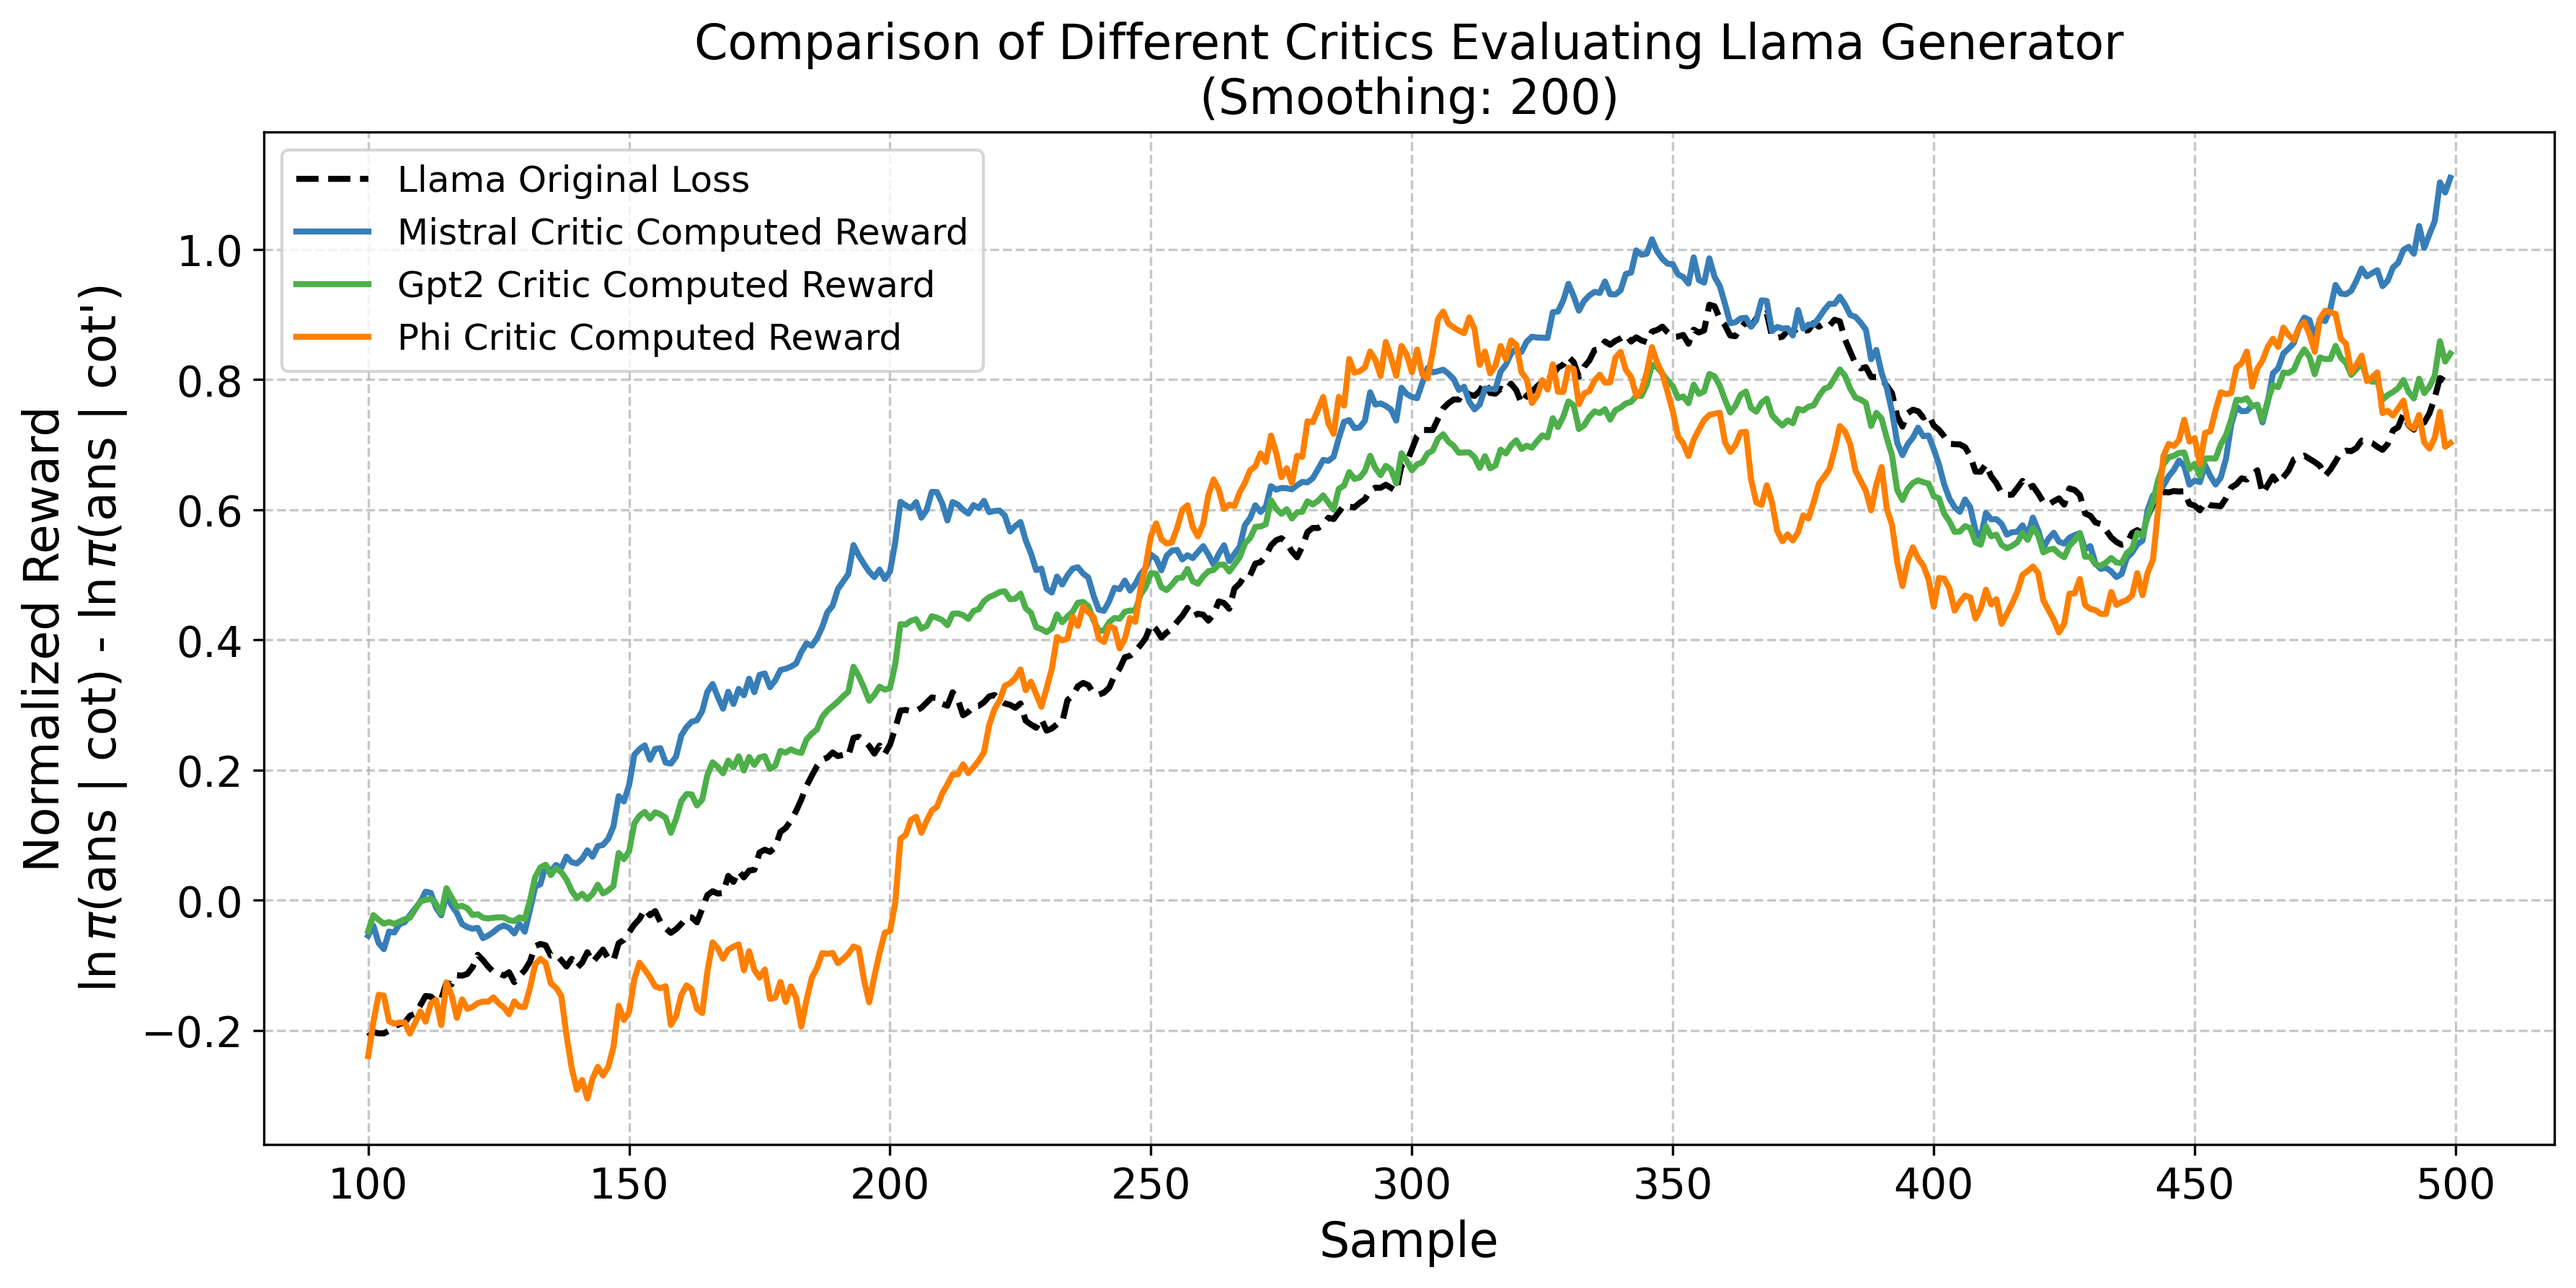
\includegraphics[width=48cm]{gsm8k_multiple_critics_comparison.png}

\vspace{0.1cm}
\raggedright
As training progresses, all critics' rewards increase in tandem: CoTs encode \textbf{transferable reasoning}, not model-specific artifacts.
}

% ===================== COLUMN 3 =====================

\posterblockM{C3A}{125,9.5}{62}{Qualitative Example: Wikipedia Continuation}{%
\textbf{Task:} condition on 200 tokens of Wikipedia, generate 50 tokens of CoT, predict next 100 tokens.

\vspace{0.3cm}
\fcolorbox{gray!60}{blue!5}{%
\parbox{58cm}{%
\textbf{Input passage (200 tokens):}
``Apoptosis (from \ldots) is a form of programmed cell death that occurs in multicellular organisms and in some eukaryotic, single-celled microorganisms such as yeast.
Biochemical events lead to characteristic cell changes (morphology) an''
}}

\vspace{0.4cm}
\fcolorbox{mkgreen}{mkgreenlight}{%
\parbox{58cm}{%
\textbf{Markovian CoT} (after training):\enspace
``understanding the underlying cellular processes is crucial.
Compressed text: Apoptosis is a form of programmed cell death occurring in multicellular organisms and some eukaryotic microorganisms.
Biochemical events lead to cell changes an Predicted next 50''

\smallskip
$\rightarrow$ \textbf{Compresses key content} into the CoT bottleneck.
}}

\vspace{0.4cm}
\fcolorbox{red!60}{red!5}{%
\parbox{58cm}{%
\textbf{Baseline CoT} (before training):\enspace
``The text is written in a formal and technical style, which may make it difficult for some readers to understand\ldots''

\smallskip
$\rightarrow$ \textbf{Irrelevant metacommentary} about writing style---no useful information for continuation.
}}
}

\posterblockM{C3B}{$(C3AB.south west)+(0,1.2)$}{62}{QA Perturbation Fragility}{%
Accuracy drop (Markovian $-$ Non-Markovian) under CoT corruption. Positive = Markovian relies more on CoT.

\vspace{0.3cm}
\centering
\renewcommand{\arraystretch}{1.35}
\begin{tabular}{l c c c c c c}
\toprule
\textbf{Dataset} & \textbf{CharRep} & \textbf{Delete} & \textbf{DigRep} & \textbf{TruncB} & \textbf{TruncF} & \textbf{Avg} \\
\midrule
ARC        & +0.320 & +0.424 & $-$0.004 & +0.069 & +0.439 & +0.250 \\
SVAMP      & +0.154 & +0.204 & +0.081 & +0.076 & +0.046 & +0.112 \\
GSM8K      & +0.059 & +0.069 & $-$0.013 & +0.105 & +0.044 & +0.053 \\
MMLU       & +0.056 & +0.124 & +0.004 & +0.038 & $-$0.001 & +0.044 \\
Arithmetic & $-$0.016 & $-$0.003 & $-$0.043 & +0.001 & $-$0.016 & $-$0.015 \\
\midrule
Overall & +0.115 & +0.164 & +0.005 & +0.058 & +0.102 & +0.089 \\
\bottomrule
\end{tabular}

\vspace{0.3cm}
\raggedright
\textbf{Wikipedia} (nats, not accuracy): avg $\Delta\ln P = +0.603$, confirming even stronger Markovian reliance.

\vspace{0.2cm}
\textbf{ARC} shows the clearest QA fragility (+25\,pp).
\textbf{Arithmetic} is a near-tie: both models treat every digit as load-bearing, so perturbation sensitivity is maximal for both.

\vspace{0.3cm}
\textbf{Scope \& limitations:}
\begin{itemize}\setlength{\itemsep}{4pt}
\item Claim is \textbf{informativeness}, not full faithfulness
\item Model could compute answer early and emit post-hoc CoT
\item Fragility + cross-model transfer are converging evidence, not proof
\end{itemize}
}

% Footer
\fill[white, rounded corners=4pt] (3,86.5) rectangle (187,88.5);
\node[font=\fontsize{36}{38}\selectfont] at (95,87.5) {%
  \textbf{Code:} \texttt{github.com/scottviteri/MarkovianTraining}
  \hspace{2cm}
  \textbf{Models:} Llama 3.1 8B, Mistral 7B, Qwen3 4B, Phi 3.5, GPT-2
  \hspace{2cm}
  \textbf{Tasks:} GSM8K, MMLU, SVAMP, ARC, Arithmetic, Wikipedia
};

\end{tikzpicture}
\end{document}
